\documentclass[wide]{cluu}
\usepackage{subcaption}
\usepackage{hyperref}
\usepackage{colortbl}
\usepackage{enumitem}
\useunder{\uline}{\ul}{}

\usepackage[round]{natbib}


\renewcommand{\arraystretch}{1}

\title{Latex support}
\author{Your name}
\date{} 

%%% BEGIN DOCUMENT
\begin{document}

\maketitle


\section{Introduction}
This is a \LaTeX\ file. Follow the text in \texttt{exercises.pdf}  and recreate the text as well as formatting in your own document.
\newline
\newline
Recreate this line and footnote\footnote{This is a footnote.}. Do not forget to include the newlines.

\subsection{Comments on referencing}
In order for the citations to work, either in this format: \citep{devlin2018bert} or in this format: \cite{devlin2018bert}, the following must be added at the end of the \LaTeX\ document:
\begin{verbatim}
    \bibliography{library}
\end{verbatim}
Or, if you are using the in other format, as illustrated below.
\begin{verbatim}
    \printbibliography
\end{verbatim}
This line above is already included in this template. The bibliography is created automatically from \texttt{library.bib} file you have imported from the github repository. Open the file and explore it. Add the Introduction to NLP coursebook by Jurafsky and add its reference using Google Scholar \footnote{This is a clickable link: \url{https://scholar.google.com/}}. Cite it here: [insert reference]. 

\section{Formatting}

To achieve the main purpose of the project, the following objectives were identified. 
\begin{enumerate}
\item This is one goal. 
\item This is another goal.
\item \ldots
\end{enumerate}
\newline
The experiments yielded interesting results. 
\begin{itemize}
\item \textbf{Experiment 1:} This is a result.
\item \textbf{Experiment 2:} This is another result.
\end{itemize}
Notice the gap difference between the previous bullet formatting and the one below. 

\begin{itemize}[noitemsep=0mm,topsep=0mm]
\item This is a \textit{point};
\item This is \textit{another} point.
\end{itemize}
Several conclusions were made.
\subsection{Headache cases}
\texttt{Hint}: look for cite and mathematical equations inside latex text.
\newline
\newline
As an example \cite{tversky1982similarity}\footnote{This citation mode should be easy.} provided \( w_1 \) relating to \( w_2 \), \( w_2 \) to \( w_3 \), yet \( w_1 \) and \( w_3 \) not having a semantic connection. 

\newline
\newline
The equation\textsuperscript{this is a superscript} can be expressed as illustrated in the Equation 1 below. This equation was brought to you by an equation Generator\footnote{\url{https://www.codecogs.com/latex/eqneditor.php}}.
\begin{equation}
\sqrt[N]{\prod_{i=1}^{N}\frac{1}{P({w|w-1})}}
\end{equation}

Here is some randomly generated text, used here and in the following Section. "Lorem ipsum dolor sit amet, consectetur adipiscing elit, sed do eiusmod tempor incididunt ut labore et dolore magna aliqua. Ut enim ad minim veniam, quis nostrud exercitation ullamco laboris nisi ut aliquip ex ea commodo consequat. Duis aute irure dolor in reprehenderit in voluptate velit esse cillum dolore eu fugiat nulla pariatur. Excepteur sint occaecat cupidatat non proident, sunt in culpa qui officia deserunt mollit anim id est laborum."

% \section{Create a new page}
% Under this Section, a newpage was added. However, scroll down to see more tasks.
% \newpage

\section{Figures}

Your task is to add some images. You can find \texttt{image1},  \texttt{image2} and \texttt{image3} in the folder \texttt{data} in the repository. Import and use them as illustrated in Figure 1 and Figure 2, respectively. First, add a separate image. 
\begin{figure}[ht!]
    \centering
    \caption{Try creating a caption over, then under the image}
    
\includegraphics[width=\textwidth]{data/image3.png}
    \label{fig:my_label}
\end{figure}



Now join two images as illustrated below in Figure 2 (a-b). 


\begin{figure}[ht!]
     \centering
     \begin{subfigure}{0.5\textwidth}
         \centering
          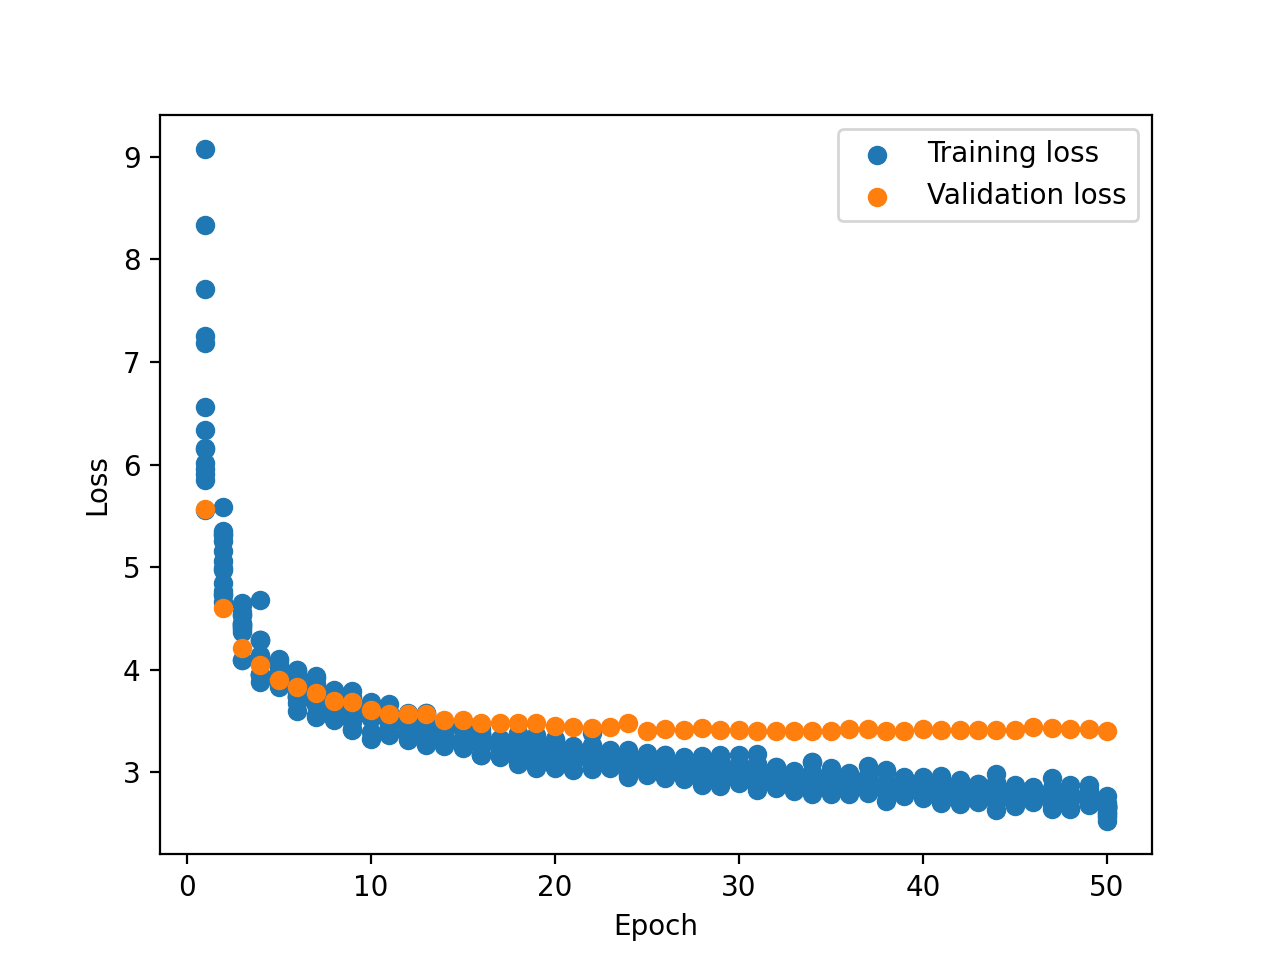
\includegraphics[width=\textwidth]{data/image1.png}
         \caption{Training and validation loss}
         \label{fig:}
     \end{subfigure}%
     \begin{subfigure}{0.5\textwidth}
         \centering
         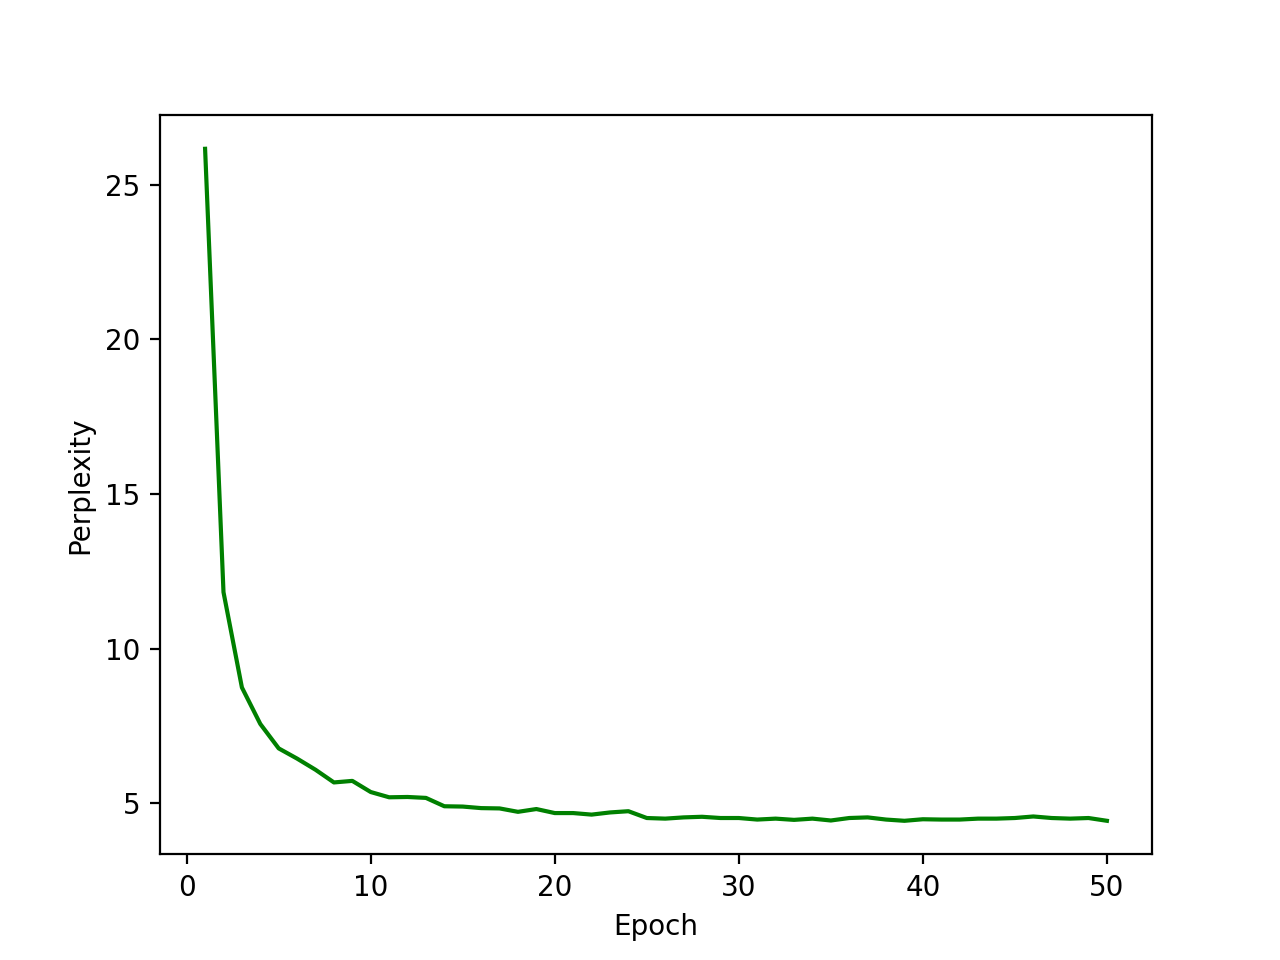
\includegraphics[width=\textwidth]{data/image2.png}
         \caption{Perplexity}
         \label{fig:transformer_bleu_original}
     \end{subfigure}
\caption{A secret model trained on a secret dataset for a secret task for 50 epochs}
\label{fig:cnn}
\end{figure}


\FloatBarrier
\newline
Next, your task is to add a table. Use a Table Generator\footnote{\url{https://www.tablesgenerator.com/}}. You can find the \texttt{table.xcls} in the folder \texttt{data} in the repository. Generate a table and add one as illustrated in Table 1, respectively.
\begin{table}[!ht]
\centering
\caption{Some randomly generated numbers}
\begin{tabular}{l|rrrr}
                   & \multicolumn{1}{l}{\textit{Model 1}} & \multicolumn{1}{l}{\textit{Model 2}} & \multicolumn{1}{l}{\textit{Model 3}} & \multicolumn{1}{l}{\textit{Model 4}} \\ \hline
\textbf{Recall}    & {\ul 99.84\%}                        & 93.43\%                              & 96.88\%                              & 90.84\%                              \\
\textbf{Precision} & 95.32\%                              & {\ul 99.09\%}                        & 90.32\%                              & {\ul 99.24\%}                 
\end{tabular}
\end{table}

\section{Paragraphs}
Recreate different paragraph speparation styles.

\subsection{Parahraph separation style no.1}

"Lorem ipsum dolor sit amet, consectetur adipiscing elit, sed do eiusmod tempor incididunt ut labore et dolore magna aliqua. Ut enim ad minim veniam, quis nostrud exercitation ullamco laboris nisi ut aliquip ex ea commodo consequat. Duis aute irure dolor in reprehenderit in voluptate velit esse cillum dolore eu fugiat nulla pariatur. Excepteur sint occaecat cupidatat non proident, sunt in culpa qui officia deserunt mollit anim id est laborum."

"Sed ut perspiciatis unde omnis iste natus error sit voluptatem accusantium doloremque laudantium, totam rem aperiam, eaque ipsa quae ab illo inventore veritatis et quasi architecto beatae vitae dicta sunt explicabo. Nemo enim ipsam voluptatem quia voluptas sit aspernatur aut odit aut fugit, sed quia consequuntur magni dolores "

"Lorem ipsum dolor sit amet, consectetur adipiscing elit, sed do eiusmod tempor incididunt ut labore et dolore magna aliqua. Ut enim ad minim veniam, quis nostrud exercitation ullamco laboris nisi ut aliquip ex ea commodo consequat. Duis aute irure dolor in reprehenderit in voluptate velit esse cillum dolore eu fugiat nulla pariatur. Excepteur sint occaecat cupidatat non proident, sunt in culpa qui officia deserunt mollit anim id est laborum."



\subsection{Parahraph separation style no.2}

"Lorem ipsum dolor sit amet, consectetur adipiscing elit, sed do eiusmod tempor incididunt ut labore et dolore magna aliqua. Ut enim ad minim veniam, quis nostrud exercitation ullamco laboris nisi ut aliquip ex ea commodo consequat. Duis aute irure dolor in reprehenderit in voluptate velit esse cillum dolore eu fugiat nulla pariatur. Excepteur sint occaecat cupidatat non proident, sunt in culpa qui officia deserunt mollit anim id est laborum."
\newline
\newline
"Sed ut perspiciatis unde omnis iste natus error sit voluptatem accusantium doloremque laudantium, totam rem aperiam, eaque ipsa quae ab illo inventore veritatis et quasi architecto beatae vitae dicta sunt explicabo, totam rem aperiam, eaque ipsa quae ab illo inventore veritatis et quasi architecto beatae vitae dicta sunt explicabo."


\bibliographystyle{plainnat}
\setlength{\bibsep}{7pt}
\bibliography{library}

\end{document}
